\documentclass[a4paper,10pt]{exam}
\usepackage[latin9]{inputenc}
\usepackage[cyr]{aeguill}
\usepackage[francais]{babel}
\usepackage{fullpage}
\usepackage{array}
\usepackage{verbatim}
\usepackage{graphicx}
\usepackage{amsmath}

\ifthenelse{\equal{\detokenize{correction}}{\jobname}}
{\printanswers}
{\noprintanswers}

\title{Architecture des ordinateurs - TD 03}

\author{}
\date{}

\begin{document}
\maketitle

\section{Position du bit à 1 le plus à gauche}
\begin{enumerate}
  \item Écrire une fonction C qui retourne la position du bit à 1
    le plus à gauche dans un mot de 32 bits en utilisant une boucle
    et l'opérateur \verb!>>!. Quel est le nombre maximum d'itérations
    effectuées ?
    \begin{solution}
\begin{verbatim}
char premier_bit_a_un(uint32_t M) {
    char pos = 0;
    while(M) {
       M = M >> 1;
       pos++;
    }
    return pos;
}
\end{verbatim}
    \end{solution}
  \item Nous souhaitons accélérer l'algorithme en utilisant une méthode
    de recherche dichotomique, dont l'algorithme est donné ci-dessous:
    \begin{enumerate}
      \item Soit un mot $M$ composé de $n$ bits. On coupe le mot en deux
        parties: $M_g$ qui contient les $n/2$ bits les plus à gauche et $M_d$
        qui contient les $n/2$ bits les plus à droite.
      \item Si $M_g = 0$ alors le bit à 1 le plus à gauche est contenu dans
        $M_d$ et sa position est comprise entre $0$ et $n/2$. On recommence
        ce processus en remplaçant $M$ par $M_d$.
      \item Si $M_g > 0$ alors le bit à 1 le plus à gauche est contenu dans
        $M_g$ et sa position est comprise entre $n/2$ et $n$. On recommence
        ce processus en remplaçant $M$ par $M_g$.
    \end{enumerate}

    Écrire cet algorithme en C. Pour sélectionner la partie gauche d'un mot de
    32 bits vous pouvez utiliser l'opération \texttt{M \& 0xFFFF0000} par exemple
    ou un décalage \verb!M >> 16!.

    \begin{solution}
\begin{verbatim}


uint32_t shift[5]  = {16        , 8     , 4   , 2     , 1   };

char premier_bit_a_un_dichotomique(uint32_t M) {
    char pos = 0;
    char i;

    for (i = 0; i <= 4; i++) {
       uint32_t Mg = M >> shift[i];
       if (Mg) {  // le bit a un est dans Mg
          M = Mg; // on remplace M par Mg
          pos += shift[i];   // on réajuste la position
                             // (on aurait pu utiliser |=)
       }
    }

    return pos;
}


uint32_t masque[5] = {0xFFFF0000, 0xFF00, 0xF0, 0b1100, 0b10};
uint32_t shift[5]  = {16        , 8     , 4   , 2     , 1   };

char premier_bit_a_un_dichotomique(uint32_t M) {
    char pos = 0;
    char i;

    for (i = 0; i <= 4; i++) {
       if (M & masque[i]) {  // le bit a un est dans Mg
          M = M >> shift[i]; // on remplace M par Mg
          pos += shift[i];   // on réajuste la position
                             // (on aurait pu utiliser |=)
       }
    }

    return pos;
}
\end{verbatim}
    \end{solution}

\end{enumerate}

\section{Code 2 parmi 5}

Un code 2 parmi 5 représente chaque chiffre de 0 à 9 sur 5 bits.
  Chaque mot de 5 bits a exactement 2 bits à 1 (d'où le nom). Voici un
  exemple de code 2 parmi 5 :
  \begin{center}
  \begin{tabular}{rl}
    0&	01100\\
    1&	11000\\
    2&	10100\\
    3&	10010\\
    4&	01010\\
    5&	00110\\
    6&	10001\\
    7&	01001\\
    8&	00101\\
    9&	00011\\
  \end{tabular}
  \end{center}
  Par la suite, on notera $C_n$ le code pour le chiffre $n$.

\begin{enumerate}

\item Le code 2 parmi 5 peut-être utilisé pour encoder des codes barres. En
  utilisant la table ci-dessus, lire la valeur du code barre suivant :
  \begin{center}
  
\includegraphics{code-barre.png}
  \end{center}

  \begin{solution}
    19889
  \end{solution}

\item La distance de Hamming $d(M,N)$ entre deux mots $M$ et $N$ représente le
  nombre de bits différents entre les mots. Par exemple, $d(1001, 1010) = 2$.
  Calculer $d(C_6, C_9)$ et $d(C_5, C_6)$.
  \begin{solution}
    $d(C_6, C_9) = 2$

    $d(C_5, C_6) = 4$
  \end{solution}

\item La distance de Hamming $d_C$ d'un code est définie comme la plus petite
  distance de Hamming possible entre deux mots distincts du code, soit $d_C = min
  \{\forall i \neq j, \quad d_h(C_i,C_j) \}$. Quelle est la distance de Hamming
  pour le code 2 parmi 5 ?

  \begin{solution}
    Soit $C_i$ et $C_j$ deux mots du code distincts. On sait que $C_i$ et $C_j$
    ont exactement deux bits à 1.

    Soit $n_i < m_i$ les positions des bits à 1 de $C_i$ et $n_j < m_j$ les position
    des bits à 1 de $C_j$.

    Premier cas : $n_i = n_j$ et $m_i = m_j$ impossible car $C_i$ et $C_j$
    distincts.

    Deuxième cas: un bit à 1 partagé par $C_i$ et $C_j$ et un bit différent.
    Supposons ici sans perte de généralité $m_i \neq m_j$. Alors la distance de
    Hamming est 2, il faut pour passer de $C_i$ à $C_j$ éteindre $m_i$ et
    allumer $m_j$.

    Troisième cas: aucun bit à 1 partagé, la distance de Hamming est
    4, il faut pour passer de $C_i$ à $C_j$ éteindre $m_i$ et $n_i$ puis allumer
    $m_j$ et $n_j$.

    Donc $d_C = min(2,4) = 2$.
  \end{solution}

\item La distance de Hamming d'un code permet de calculer combien d'erreurs
  peuvent être détectées $e_d$ et combien d'erreurs peuvent être corrigées $e_c$.
  On définit $e_d = d_C - 1$ et $e_c = \lfloor \frac{d_C-1}{2} \rfloor$.
  Combien d'erreurs peuvent être détectées par le code 2 parmi 5 ?
  Combien d'erreurs peuvent être corrigées ?

  \begin{solution}
    $e_d = 2-1 = 1$ et $e_c = 0$.
  \end{solution}
\end{enumerate}

\section{Code avec bit de parité}
On veut envoyer des mots ($a_3\dots a_0$) de $4$ bits sur un canal. Le code de parité consiste
à ajouter un bit $p$ devant le mot $pa_3\dots a_0$ qui signale la parité de la
somme des bits du mot ($p = a_3 \oplus a_2  \oplus a_1 \oplus a_0$). Si la somme est paire,
$p = 0$, sinon $p = 1$.

\begin{enumerate}
\item Encoder les mots $1010$ et $1000$ avec un bit de parité.
\begin{solution}
  $0 1010$

  $1 1000$
\end{solution}
\item Calculer la distance de Hamming du code avec bit de parité.
\begin{solution}
  \begin{itemize}
  \item Prenons deux mots consécutifs du code: $00000$ et $10001$,
    $d_h(00000,10001) = 2$, donc $d_c \leq 2$.

  \item Soit deux mots de 4 bits distincts $x$ et $y$,
    \begin{itemize}
      \item Si $d_h(x,y) \geq 2$ alors $d_h(parite(x), parite(y)) \geq 2$.
      \item Si $d_h(x,y) = 1$ alors $parite(x) \neq parite(y)$ donc
        $d_h(parite(x), parite(y)) = 2$
    \end{itemize}

  \item Dans tous les cas $d_h \geq 2$ donc $d_c = 2$.
  \end{itemize}
\end{solution}

\item Combien d'erreurs peuvent être détectées ? Combien peuvent être
    corrigées ?
\begin{solution}
  On peut détecter $2-1=1$ erreur et on ne peut en corriger aucune.
\end{solution}
\end{enumerate}

\section{Code à répétition}
Le code à répétition 3 consiste à remplacer chaque 0 du mot initial
par 000 et chaque 1 par 111.

\begin{enumerate}
  \item Calculer la distance de Hamming du code à répétition 3.
    \begin{solution}
      Il n'y a que 2 mots dans l'image du code, 000 et 111, la distance est 3.
    \end{solution}
  \item Combien d'erreurs peuvent être détectées ? Combien peuvent être
    corrigées ?
    \begin{solution}
      $3-1 = 2$ erreurs peuvent être détectées. $\frac{2}{2} = 1$ erreur
      peut être corrigée.
    \end{solution}
  \item Vous recevez les messages suivants :

    $111000111$

    $110000011011$

    Indiquez si des erreurs se sont produites et corrigez-les le cas échéant.
    \begin{solution}
      premier message : pas d'erreur.
      deuxième message : 3 erreurs, $111000111111$
    \end{solution}

  \item Vous disposez d'un canal de communications dont la probabilité
    d'intervertir un bit du message est de $p_e = 0.001$ (pour tout $n$ et $m$
    distincts les probabilités d'avoir une erreur sur le bit $n$ et une erreur sur
    le bit $m$ sont considérées indépendantes). Vous utilisez un code à
    répétition 3 pour envoyer un message original de $100$ bits. Quelle est la
    probabilité pour que le destinataire reçoive le bon message avant correction
    ? Après correction ?

    \begin{solution}
        Soit $N_n$ la loi donnant le nombre d'erreurs pour un message de longueur $n$.
        $N_n$ suit une loi binomiale (car les erreurs sont des évènements
        indépendants). Donc $P(N_n = k) = C_n^k.p_e^{k}.(1-p_e)^{(n-k)}$.

      \begin{itemize}
        \item La probabilité d'avoir un bon message avant correction, c'est
          $P(N_{300}=0) = C_{300}^0.p_e^0.(1-p_e)^{300} = (1-p_e)^{300} > 0.73$

        \item Soit $P_1$ a probabilité d'avoir une ou zéro erreur par bloc de trois bits:
          $ P_1 = P(N_3=1) + P(N_3=0) = 3.pe.(1-p_e)^2 + (1-p_e)^3$

          Donc la probabilité de pouvoir corriger un bloc de trois bits
          est de : $P_1$.

          La probabilité de pouvoir corriger le message composé de $100$
          blocs est de
          $(P_1)^{100} > 0.9997$
        \end{itemize}
    \end{solution}
\end{enumerate}

\section{Code de Hamming (7,4)}
Le code de Hamming (7,4) transmet 4 bits d'informations en utilisant 3 bits de
parité.
Pour encoder le mot $a_3a_2a_1a_0$ on écrira $p_1p_2a_0p_3a_1a_2a_3$
avec $p_1 = a_0 \oplus a_1 \oplus a_3$, $p_2 = a_0 \oplus a_2 \oplus a_3$
et $p_3 = a_1 \oplus a_2 \oplus a_3$.

On peut résumer la couverture des bits de parité avec la table
ou avec le diagramme de Venn suivants :

\begin{center}
  \begin{minipage}{0.4\textwidth}
\begin{tabular}{lcccc}
      & $a_0$ & $a_1$ & $a_2$ & $a_3$ \\
$p_1$ &   1   &   1   &   0   &   1   \\
$p_2$ &   1   &   0   &   1   &   1   \\
$p_3$ &   0   &   1   &   1   &   1   \\
\end{tabular}
\end{minipage}
\begin{minipage}{0.4\textwidth}
  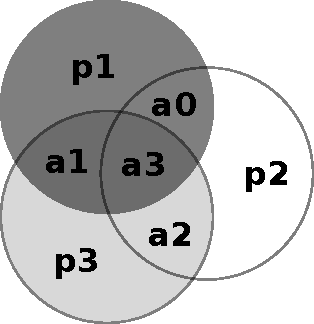
\includegraphics[width=3cm]{venn-hamming}
\end{minipage}
\end{center}

\begin{enumerate}
  \item En s'appuyant sur le diagramme de Venn, si l'on change un bit des données
    ($a_0$ à $a_3$), combien de bits de parité changent nécessairement ?
    \begin{solution}
      2 ou 3 (pour $a_3$)
    \end{solution}
  \item Quelle est donc la distance de Hamming du code ? Combien d'erreurs
    peuvent être détectées ? Combien peuvent être corrigées ?
    \begin{solution}
      La distance de Hamming du code est $2+1 = 3$. On peut donc détecter $2$ erreurs et en
      corriger $1$.
    \end{solution}

  \item Vous recevez les messages suivants :
  
    $0001111$
    
    $1110010$
    
    $1101110$
    
    $0011111$.
    
    Indiquez si une erreur s'est produite et corrigez le mot reçu le cas échéant.
    \begin{solution}
      $0001111$ Message correct (vérifier que le diagramme de Venn est correct).

      $1110010$ p3 et p2 sont incorrects, pour rendre le message correct en
      changeant un seul bit, il faut changer a2. On remarque que $3+2 \equiv 2
      [3]$.

      $1101110$ p3 est incorrect, erreur sur le bit de parité.

      $0011111$ p1 et p2 incorrects, il faut changer a0. On remarque que $1+2
      \equiv 0 [3]$.
    \end{solution}



\end{enumerate}



\end{document}
